\section{Applications}
%按应用领域分了,再统计一下
This section introduces prevalent application domains where Design-by-Analogy can deploy and examines domain-specific challenges, focusing on three sectors: Creative Industries, Intelligent Manufacturing, Education and Service Industries. Although DbA methods could theoretically support creative processes in other domains (e.g. pharmaceutical design, algorithmic design), this study exclusively addresses end-to-end applications that directly serve users and solve practical problems.
% 在本节中,我们介绍了常见的类比设计应用领域,并讨论了每个应用领域特有的分析挑战。这包括三个领域:创意工业, 智能制造,以及教育及服务工业。虽然其他应用领域也可使用design by analogy方法进行创造过程的辅助(如医药领域的药品设计,生物化学领域中的基于类比启发新化合物形式,算法设计领域的根据类比设计新算法),但它们不在本文的讨论范围内。在本节中,我们关注可以直接服务用户,解决实际的问题的端到端产业和行业上的应用。
\subsection{Creative Industries} %【13篇】
In 1998, the UK Department for Culture, Media and Sport (DCMS) defined ``creative industries'' as \textit{``Based upon activities which have their origin in individual creativity, skill and talent, and as having the potential for wealth creation through the generation and exploitation of intellectual property}\cite{miles2008hidden}. '' The Design-by-Analogy Application cases collected in this paper include creative writing, graphic design, product design, 3D modeling, animation, web design, scientific tasks, data visualization and the function of computer aided design system which related to computer graphics development, researchers using DbA methods toward different domain challenges, excluding film and music. Industrial outputs rely primarily on computational technologies and structured data, barring noncreative factors(e.g., political or force majeure events) \cite{miles2008hidden}. Our investigation identifies two core challenges for novices the create process: (1) The prevalent high technical and aesthetic barriers in software requiring experience-creativity synergy, frequently preventing concept realization\cite{hsueh2024counts}. It is common for novice designers to have an idea but be unable to implement it through software or implement it imperfectly. (2) Trendy aesthetic, emerging cultures, and edge-cutting concepts is uneven dissemination, due to the universal aesthetic knowledge bases, creative knowledge bases, design theory bases, and etc. still lacking of universal tool embedded. The effective integration of DbA technologies can: (1) Enable beginners and professionals to rapidly access cutting-edge design knowledge (patent details, case imagery, semantic inspiration). (2) Facilitate precise transfer of knowledge, styles, and content to enhance creative representation and efficiency. (3) Stimulate creator innovation through intrinsically guided knowledge exploration, thereby reinforcing creative autonomy. Academic research\cite{srinivasan2024improving, masson2025textoshop, warner2023interactive, chen2024beyond,wang2024reelframer, zheng2024disciplink,yan2023xcreation,chen2021umitation, kittur2019scaling, goucher2019crowdsourcing, han2018computational, lin2025inkspire, song2020exploration} has proposed domain specific solutions detailed subsequently.


%1998年,文化、媒体和体育部(DCMS)将创意产业定义为基于源自个人创造力、技能和天赋的活动,并且具有通过创造和开发知识产权来创造财富的潜力。本文所收集到的类比设计案例,涵盖创意内容写作、平面设计、产品设计、3d模型设计、动画设计、网站设计、科研任务、数据可视化设计及相关计算机辅助设计软件(CAD)的相关图形学功能开发等,尚未涵盖电影、音乐。本行业的工业化产出几乎仰赖于计算机技术和结构化的数据,除了非创造过程以外的其他因素如政治、不可抗力因素等,我们调查了相关研究发现本行业初学者在创造过程中的一些痛点,其中:大量的软件有着高使用门槛和美学门槛,这些门槛往往需要经验和创意的共同加持,新手设计师有一个idea但无法通过软件进行实现或者实现的不完善的情况是常态。第二点,潮流美学趋势、新兴文化、前沿理念在知识密集的区域会大面积传播,普适的软件内嵌美学知识库,创意知识库,设计数据库等通过类比设计这一机制可以促进地区的文化平权。类比设计的技术的有效整合可以(1)使不同知识深度的操作者可以快速链接到前沿知识,如相关的专利的具体设计细节,案例图片,近距离或远距离的词语启发等;(2)基于结构化映射计算,软件自动化的对知识、图形,风格等内容进行映射和迁移,从而辅助操作者更准确和更高水平的展现创意,提升完成度和效率,人辅助;(3)创意类比可以激发作者的创造力,根据作者的内在经验和知识来驱动外部知识的发散方向,这有利于保护和增强作者的内在价值和主体感。在学术研究中,学者们已经使用了各种解决方案来应对这些挑战【13篇】【1、4、9、10、11、13、15、32、42、43、45、50、71、】,我们根据应用领域的不同在下文对其方法进行详细描述。


%In creative product design, high cognitive load and design fixation\cite{moreno2015step} challenge ideation. \textbf{\textit{Crowdsourcing Inspiration}} employs crowdsourcing and text mining to extract semantic patterns from solution databases, visualizing word frequency distributions\cite{goucher2019crowdsourcing, kittur2019scaling}. \textit{\textbf{Analogilead}} enables chunk-based recombination for scalable analogical exploration\cite{srinivasan2024improving}. \textit{\textbf{The retriever}} proposes 16 ontology-based relations. By abstract the ontology relations, it retrieving and constructing an ontology or its substructure\cite{han2018computational}.
%在产品创意设计领域,一个idea的诞生需要保证创造性的同时考虑大量复杂性因素,这一过程的认知负荷很高,且极容易陷入设计固定,【42】通过众包方法得到关于12个设计问题的大规模解决方案文本,并且对解决方案进行文本挖掘,以沿频率域提取单词,映射为语义距离,并可视化展示给设计师增强创造力,【43】Kittur等人利用人群协作和AI来扩展类比创新,通过将类比过程分解为抽象、搜索和应用三个步骤,并分配给不同的人类和机器处理器,从而在这一阶段解决设计固定。【1】analogilead则通过设计师自主的组块和重组扩展类比规模,回应这一挑战。【45】The retriever 提出了16种基于本体的关系,通过在不太熟悉的本体(目标本体)中基于已知术语 C 以及从熟悉的本体(基础本体)中的 A:B 抽象出的本体关系,检索未知的 X 或多个 X,来构建一个本体或本体的一部分,激发创意。
%For graphic and 3D design, style modification typically requires rebuilding geometries from foundational elements. \textit{\textbf{VST}} allowing designers to define element correspondences and style attributes\cite{warner2023interactive}.
%automating vector graphic style transfer while preserving artistic intent of designer
%在平面设计和3d设计领域,图形和模型风格的改变往往意味着操作者需要弃用之前做的内容并重新在软件中从点、线、面开始制作新的形状,【9】warner等人在尊重设计师品味以及风格迁移所固有的主观性的同时利用自动化方法,设计师在其界面上可以调整跨设计元素的对应关系,并自定义要更改的风格属性,通过生成式人工智能迁移和映射矢量图形的风格,优化冗余步骤。
%In creative software development, transferring experience based on culture, user behavior, interaction, etc. often leads to product innovation. \textbf{\textit{Textoshop}} innovates by transferring image editing logic to text manipulation: words as pixels, sentences as regions, and tone as color\cite{masson2025textoshop}.
%This application enabling novel textual operations through transfered interaction
%在计算机辅助创意的软件开发过程中,基于文化、用户行为、交互等内容进行经验的迁移往往会带来产品的创新,【4】Textoshop利用图片编辑的逻辑迭代文字编辑,他们将单词视为像素,句子视为区域,语气视为颜色。对文本的直接操作可移动、缩短、扩展和重新排列文本;工具可改变数量、时态和语法;在色调选择器中,颜色映射到沿三个维度探索的语气;而图层则有助于组织文本并进行版本管理等。
%In journalistic content creation, the rapid expansion and transformation of content forms usually require the switching of diverse disciplinary skills. \textit{\textbf{ReelFramer}}, converting print articles into short video scripts using 3 different narrative frameworks\cite{wang2024reelframer}. \textbf{\textit{Xcreation}} \cite{yan2023xcreation} transform text-to-illustration workflows through editable entity relationship graphs.
%在新闻内容创作领域,新闻内容形式的快速扩展和转化通常需要差异性的学科技能切换,wang等人【11】提出三种适用于短片的叙事框架,这些框架既适应社交媒体规范,又保留了新闻价值,每种框架在信息和娱乐之间有着不同的平衡,他们的ReelFramer可帮助记者将印刷文章根据规则映射为脚本和故事板。相似的模态转换,还有在插画设计领域中的文字模态到图片插图模态的转换,yan等人【15】整合了一个可解释的实体关系图,以直观地表示图片元素及其之间的关系,从而将文字到图片的这种映射规则可视化成为具有边、节点的图,用户可以编辑,提高映射的可用性。
%For web design, front-end UI development involves highly repetitive DOM modifications requiring constant contextual adaptation. \textbf{\textit{Umitation}} optimizes repetitive DOM adjustments by recording UI behaviors on source sites and mapping changes to target elements, contextualizing design adaptations.
%在网页设计中,大量的前端ui文档对象模型的变化设计工作是重复性高且需不断根据情境调整的,一次ui行为更改和调整意味着复杂的底层内容变动,基于经验、可行性和情境进行设计则会提升效率,umitation【32】帮助设计师提取、编辑并将前端 UI 行为示例适配到目标网站的系统。通过首先在源网站上指定一个或多个源元素,然后通过与它们交互来记录其行为。umitation将自动捕获文档对象模型(DOM)的变化并将其映射到目标网站上的合适元素,帮助明确设计师所需的ui行为。
%In data visualization, achieving user comprehension of complex data and developing more comprehensible representations is the primary objective. \textbf{\textit{AnalogyMate}} employs proportional text and graphics for data analogy to convey complex numerical values, units, and concepts in ways that enhance comprehension\cite{chen2024beyond}.
%在数据可视化设计中,用户对复杂数据的清晰理解是首要目标,而给复杂数据寻找更具理解力的表征是难点,chen等人【10】利用与数据比例一致的文字和图像来进行数据类比,他们定义了数据类比设计的多种维度,致力于将复杂的难以理解的数值、单位、概念以更能增加理解的方式传达给读者。
%In interdisciplinary research, cross-disciplinary information retrieval involves terminology discrepancies and integration of vast content. \textbf{\textit{DiscipLink}} assist users in query formulation, automatically expanding queries using domain-specific terms, extracting topics, and establishing research connections\cite{zheng2024disciplink}.
%在跨学科科研中,跨学科的信息搜索意味着术语差异,大量内容的整合对比,陌生学科的高度分散的知识中进行梳理是一项重大挑战,DiscipLink【13】从辅助用户提问出发,根据特定学科术语自动扩展查询、从检索到的论文中提取主题以及与问题之间的联系,帮助用户进行跨领域的术语转换和科研内容映射。




\subsection{Intelligent Manufacturing} %智能制造,会写生物设计,机械设计,农业,电子电路还有机器人什么的(制造的)【15篇】
In the Industry 4.0, intelligent manufacturing is defined as an advanced mode that utilizes artificial intelligence, the Internet of Things, cyber-physical systems, and related technologies to transform traditional manufacturing resources into intelligent objects with perception, decision-making, and collaboration capabilities. This enables data-driven flexible production for mass customization.\cite{zhong2017intelligent, jiang2022data, li2017applications}. We documents DbA applications including: knowledge-based design inspiration\cite{kang2025biospark}, case-integrated design-to-manufacturing lifecycle system\cite{thomas2013extending, schulz2014design}, case-based cyber-physical system\cite{gonzalez2018energy}, and process-oriented intelligent knowledge transfer\cite{emerson2024anther}. These span manufacturing method design\cite{luo2019computer}, product innovation\cite{liu2023smfm}, smart sensor/wearable device development\cite{hong2024fishbone}, plastics processing\cite{khosravani2022intelligent}, chemical/pharmaceutical synthesis\cite{coley2019robotic}, and agriculture\cite{zhai2020applying}. DbA further empowers industrial upgrading through manufacturing case libraries and design databases by: (1) Transferring cross-domain knowledge to product manufacturing methods, supporting innovative resource utilization; (2) promote lifecycle servitization of physical manufacturing resources through AI-assisted manufacturing decisions; (3) provide replicable conversion pathways for niche manufacturing techniques, fostering innovation within Community Of Practice(COP) and fostering archival and transform of ambiguous data\cite{zhong2017intelligent, kusiak2000computational, jiang2022data}. Deep exploration and integration of this mechanism in intelligent manufacturing offers beginners heuristic resources and assists experts in enhancing complex problem-solving through cross-scenario functional and structural migration. It optimizes implementation of modular production units, flexible logistics planning, and mass personalized customization\cite{li2017applications}, while improving energy and resource allocation to advance sustainable development. Research in this domain includes\cite{kang2025biospark, emerson2024anther, zhai2020applying, fan2014fractal, luo2021guiding, schulz2014design, liu2023smfm, luo2019computer, hong2024fishbone, khosravani2022intelligent, you2018design, thomas2013extending, coley2019robotic, gonzalez2018energy}.
%在工业4.0背景下,智能制造可定义为依托人工智能、物联网、信息物理系统等技术,将传统制造资源转化为具备感知、决策与协作能力的智能对象,通过数据驱动与柔性化生产实现大规模定制的先进制造模式。本文收集的类比设计相关应用涵盖基于知识库的设计灵感启发、基于案例集成设计到制造全生命周期、基于案例的信息物理系统、基于知识的流程规划、基于工艺的智能知识迁移等,包含的应用领域包括制造方法设计,产品创新设计,智能传感器与可穿戴设备的设计与制造,塑料加工,化学合成与制药、农业等行业。类比设计在该领域的应用可进一步赋能产业升级,通过构建制造案例库与设计数据库:(1)能将生物结构、工程专利等跨领域知识迁移至产品制造方法中,促进制造资源的创新应用;(2)基于工艺规划经验与知识数据库,结合AI辅助制造决策,推动实体制造资源的全生命周期服务化;(3)为小众制造技艺提供可复刻的转换路径,促进实践制造社区的创新和模糊数据存档。在智能制造领域深入探讨这种机制并集成,可为初学者提供工艺参数、经验库等启发资源,帮助专家通过功能、结构等内容的跨场景迁移提升复杂问题的解决效率,依托创意类比设计优化模块化生产单元设计、柔性物流路径规划,大规模个性化定制等创新场景的落地,优化能源和资源分配,促进智能制造行业的可持续发展。在学术研究中,学者们已经使用了各种解决方案来应对这些挑战【2,3,12,30,41,52,57,61,62,64,67,72,77,80,82】,我们根据应用场景的不同在下文对其方法进行详细描述。
%---------------------------
%智能制造行业关注的三个内容(1)流程、加工、工艺数据实时采集的完整性(如温度、振动、能耗等);(2)实体可制造资源的全生命周期服务化。(3)柔性化、个性化、定制化生产的需求在大幅增加。



%在农业智能化领域,

% 根据文档内容及所提供的文章标题,可对各研究所属行业及解决的智能制造问题分析如下:  

% 1. **《将基于案例的推理和基于学习的适应策略应用于葡萄种植中的灌溉调度》**:  
%    所属行业为农业智能化领域。其通过案例推理与学习策略优化灌溉调度,对应文档中智能制造“数据驱动决策”与“自适应控制”的技术特征,解决了农业生产中水资源高效利用的实时决策问题,类似于制造系统中基于历史数据的工艺参数优化(如文档中提到的RFID实时数据驱动生产调度,)。  

% 2. **《通过实例进行设计与制造》**:  
%    属于制造业设计领域。该研究利用实例推理辅助设计与制造,契合文档中“智能设计”与“案例库应用”的方向(如提到的基于CAD/CAM的智能原型系统),解决了产品设计中知识迁移效率低的问题,实现设计经验的复用与创新。  

% 3. **《基于功能案例建模和生物TRIZ的生物启发式设计中的设计类比》《基于SMFM的创新产品概念设计类比检索工具》**:  
%    归属产品创新设计领域。两者通过生物类比与功能建模推动设计创新,对应文档中“类比设计辅助制造”的思路(如提到的多智能体协作与跨领域知识映射),解决了传统设计中创意生成与功能优化的瓶颈,类似于将生物结构类比至机械部件设计的跨领域应用。  

% 4. **《受鱼骨和荨麻纤维启发的高灵敏度、宽传感范围可拉伸应变传感器及其在可穿戴电子设备中的应用》**:  
%    属于智能传感器与可穿戴设备制造领域。其通过生物启发的材料设计提升传感器性能,对应文档中“智能对象感知能力”的技术要求(如提到的RFID与传感器集成实现生产资源感知),解决了智能制造中实时数据采集的精度与范围问题,为柔性制造提供硬件支撑。  

% 5. **《基于智能知识的系统以改进注塑成型工艺》**:  
%    属于塑料加工制造领域。该系统通过智能知识管理优化注塑工艺,对应文档中“AI驱动的工艺优化”(如提到的AI在生产流程监控中的应用),解决了注塑成型中参数优化与质量控制的复杂性问题,实现工艺的自适应调整。  

% 6. **《类比设计:一种用于岩土工程的特征树方法》**:  
%    属于土木工程智能化领域。其将类比设计应用于岩土工程,类似于文档中“跨领域知识迁移”的思路(如提到的制造系统多智能体协作),解决了岩土工程中复杂场景的设计决策问题,为智能制造中的模块化设计提供方法论参考。  

% 7. **《扩展和自动化用于需求生成与分析的系统理论危害分析》**:  
%    属于制造系统安全与需求分析领域。其通过自动化危害分析提升系统可靠性,对应文档中“智能制造系统安全性”的考量(如提到的云计算安全挑战),解决了生产流程中潜在风险的预判与需求分析效率问题。  

% 8. **《一个由人工智能规划驱动的用于有机化合物流动合成的机器人平台》**:  
%    属于化学合成与制药制造领域。该平台通过AI驱动机器人实现自动化合成,对应文档中“智能装备与自主控制”的技术方向(如提到的智能机器人在IMS中的应用),解决了有机合成中流程复杂、自动化程度低的问题,推动制药制造向智能化转型。  

% 9. **《基于案例推理策略的能源优化》**:  
%    属于工业能源管理领域。其通过案例推理优化能源分配,对应文档中“制造资源高效利用”的目标(如提到的ICT助力制造业节能),解决了工业生产中能源消耗的优化调度问题,实现智能制造中的绿色生产需求。  

% 这些研究从不同维度呼应了文档中智能制造在“数据驱动决策、跨领域类比设计、智能装备优化、资源服务化”等方面的技术需求,通过案例推理、生物启发、AI规划等方法,分别解决了各行业中知识迁移、工艺优化、实时感知、能源效率等具体问题,为工业4.0背景下的智能制造提供了多元化的解决方案。

\subsection{Education and Service Industries}%会写一些类似服务业的内容,金融类比,服务流程类比也有一些文章【14篇】
Analogical reasoning, recognized as fundamental to learning\cite{winston1980learning} with deep philosophical roots and extensive mathematical applications, enjoys broad pedagogical exploration supported by substantial theoretical and empirical research\cite{bettin2023pedagogical}. We documents DbA applications in education, distinct from pure analogical reasoning, which structurally scaffold analogical application in educational contexts\cite{winston1980learning, bettin2023pedagogical}. By systematically retrieving knowledge, experience, and data, then transferring them via domain-specific mapping rules to target scenarios, these tools empower educators to rapidly leverage adapted resources for advancing students' conceptual understanding, metacognition, and interdisciplinary exchange\cite{karunathilaka2025intuit, chen2024BIDTrain, ball2019advancing}.
Within service industries, DbA facilitates transactional innovation across cultures, domains, services, and communities by enabling communication, collaboration, and co-creation. Such tools map and migrate tacit knowledge through domain-specific rules, allowing practitioners to integrate existing expertise with novel insights while addressing critical challenges\cite{moreno2014analogies, lee2020customized}: (1) Leveraging shared methodologies (e.g., touchpoint analysis, stakeholder mapping, service blueprints\cite{stickdorn2012service}) despite service design's case-specific nature, enabling cross-scenario inspiration through experience repositories; (2) Embedding resolved complexities from other contexts into service design applications to enhance practical efficacy; and (3) This field demands rigorous design evaluation, and DbA based assessment holds significant potential for evaluating and predicting service efficacy. Research in this domain includes\cite{chen2024BIDTrain, kim2023star, dougan2022predicting, jiayang2023storyanalogy, cao2025medai, shao2025unlock, bettin2023pedagogical, Ju2025toward, karunathilaka2025intuit, vattam2011dane, la2020designing, moreno2014analogies, lee2020customized, lupiani2017monitoring}.
%类比推理被认为是学习的本质,其深厚的哲学研究根基、在数学科学中的应用,使其在教育学界的探索十分广泛,有着大量的理论与实践研究。本文检索到的类比设计工具,区别于单纯的类比推理,旨在结构化的辅助教学场景中的类比应用,通过系统检索到的知识、经验、数据等,经由特异性映射规则迁移到具体的教育应用场景中,使教育工作者可以快速使用迁移好的知识推动学生的概念学习、元认知、理解能力等,并促进学科间交流。
%在服务工业领域,类比设计被应用于促进跨文化、跨领域、跨服务、跨社区的事务性工作创新,通过支持交流、协作与共创机制驱动价值创造。该类工具将模糊知识、经验等抽象内容基于领域特定规则进行映射迁移,赋能事务性工作者快速融合经验与新知开展工作,并针对性解决以下核心问题:1)尽管服务设计具有强情境依赖性(case by case)与在地特异性,但共性要素依然存在(如触点分析、利益相关方分析、服务蓝图等流程化方法),该层面可依托经验库实现推荐机制、灵感激发与跨场景映射;2)特定复杂性问题可能已在其他情境中被高效解决,通过将既有经验与细节嵌入服务设计理论框架及流程化交互支持系统,可强化类比设计的实践效能;4)本领域对设计评估需求很高,基于类比设计评估和预测服务效能具有很大潜力。


%
\begin{figure}
    \centering
    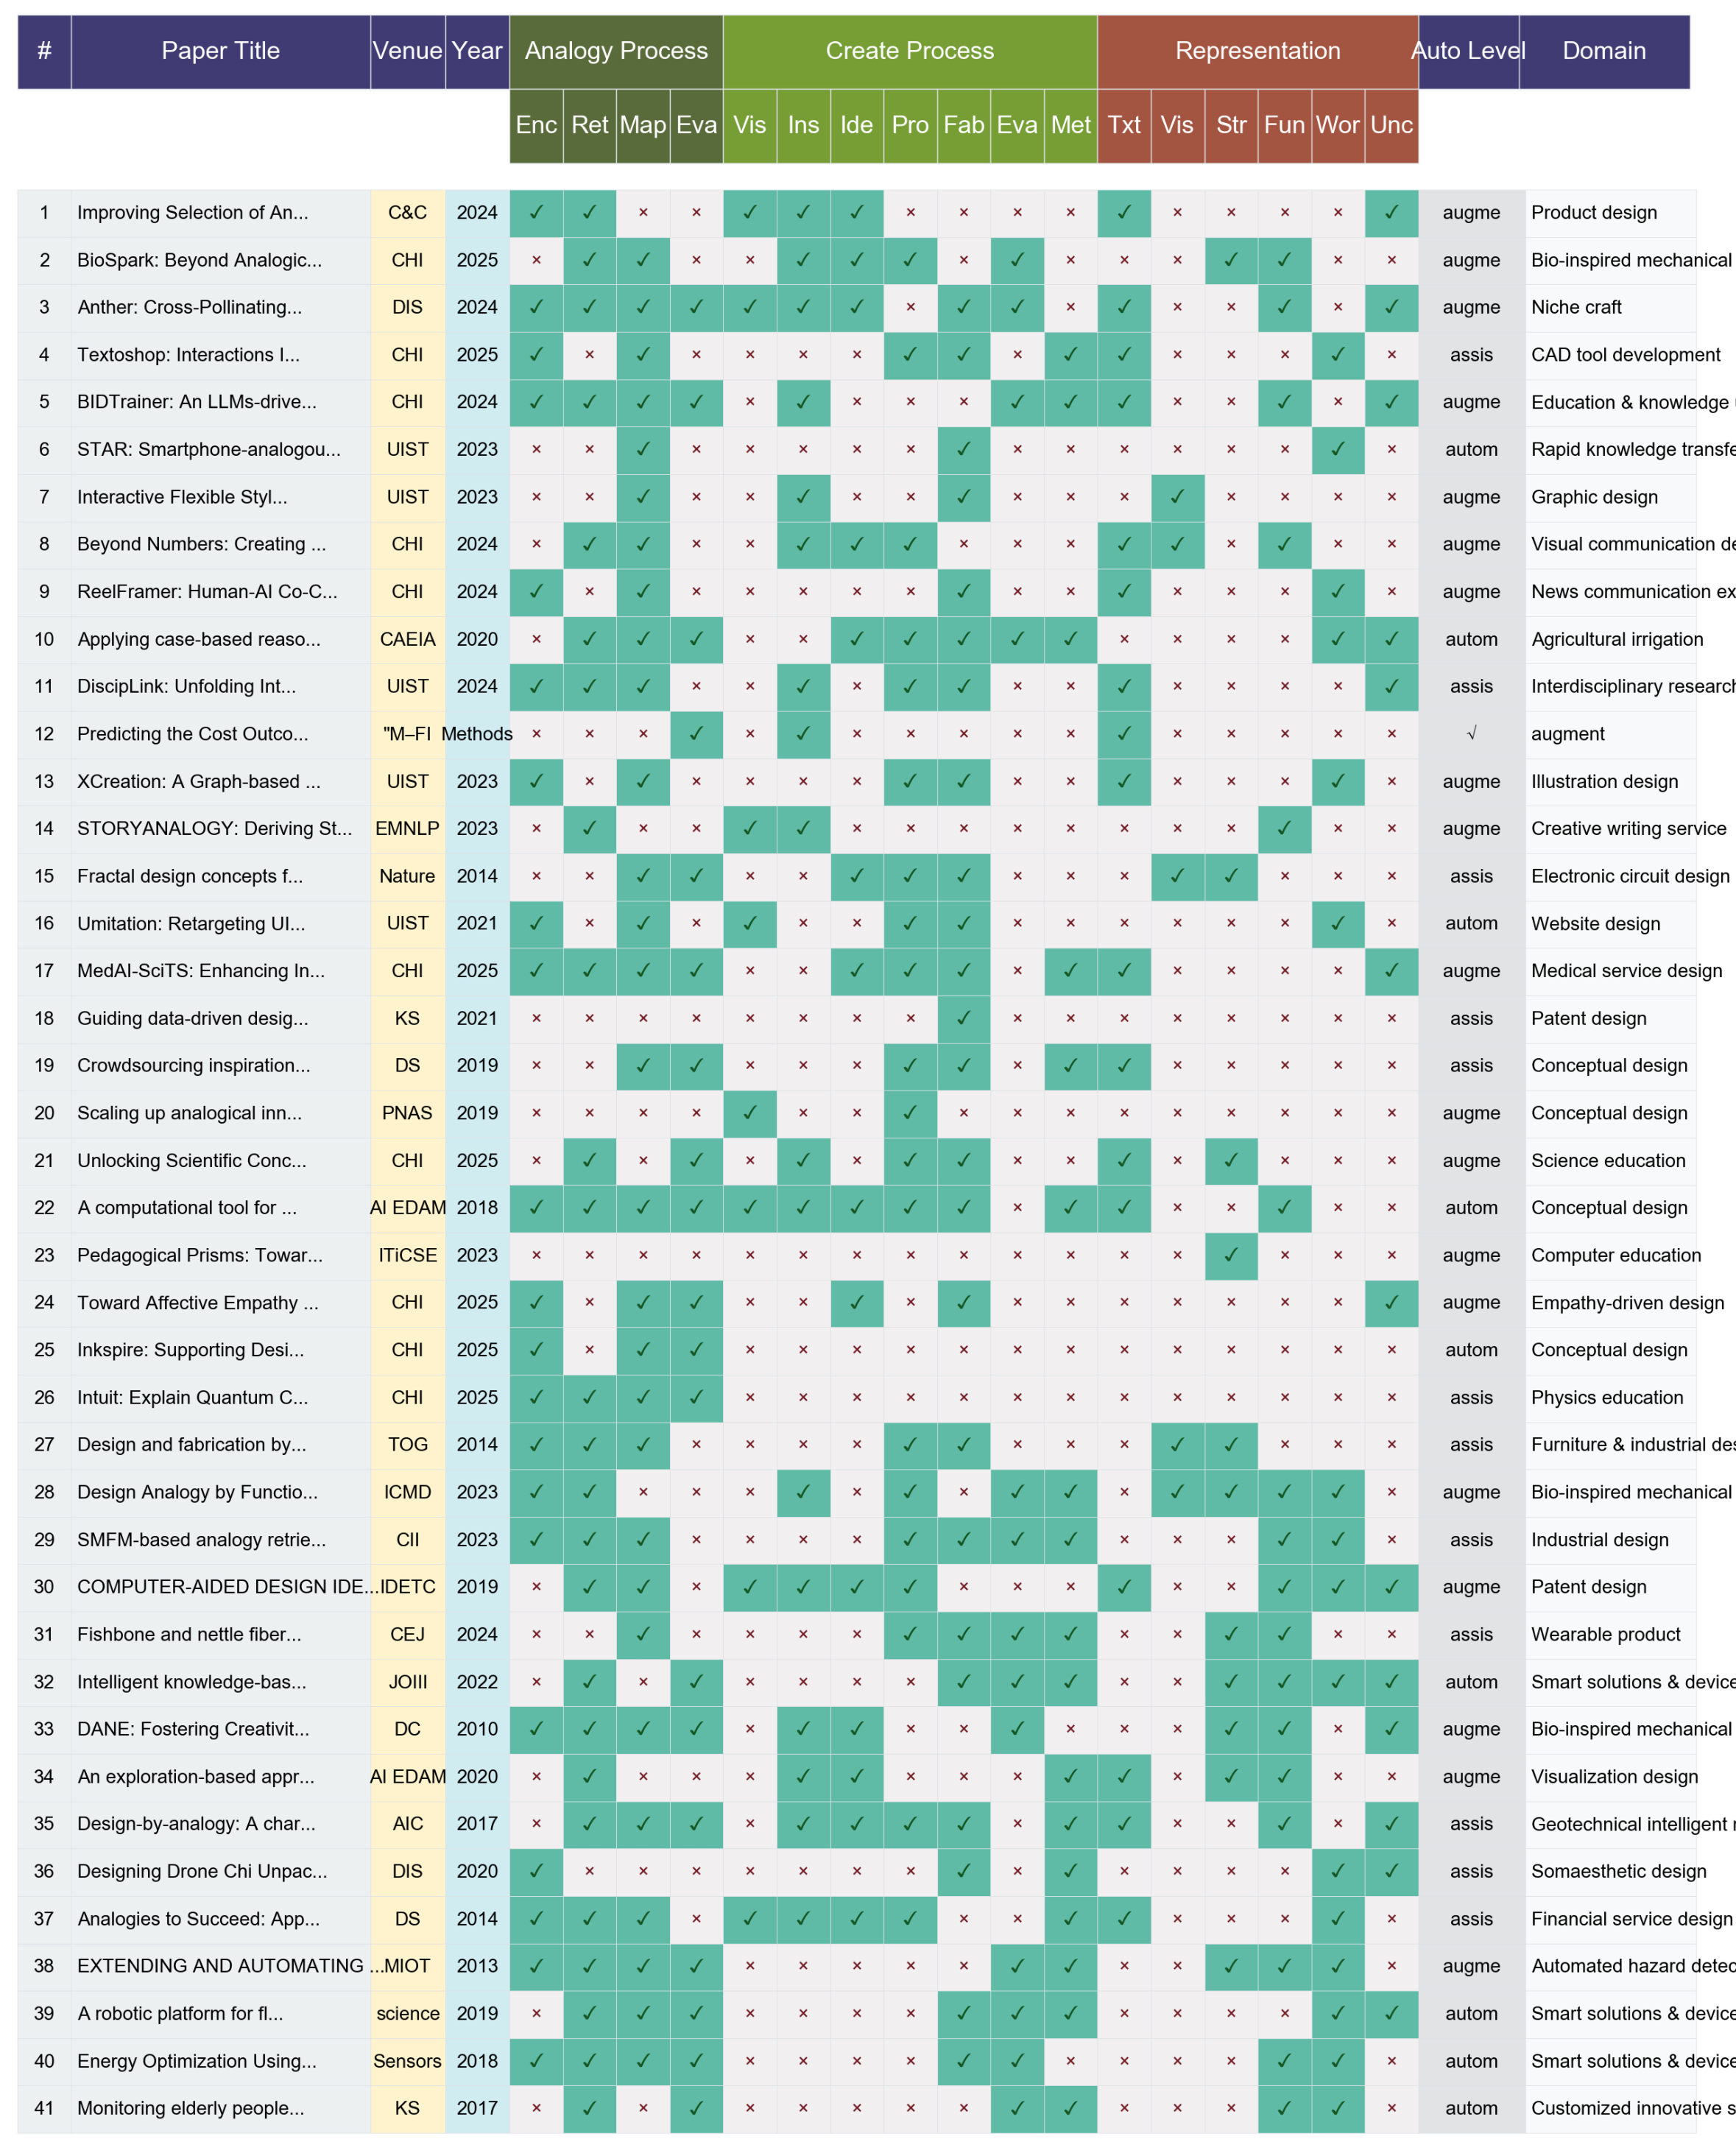
\includegraphics[width=1\linewidth]{Figures/complete_41_papers_presentation 2.png}
    \caption{This figure visualizes a taxonomic matrix consisting of 42 representative publications in the field of AI - enabled analogical design from 2010 to 2025. The x - axis represents different application domains (for example, communication design and fabrication), while the y - axis distinguishes between two technological orientations: Augment and Automate. The publication year encodes the temporal distribution, and visual markers indicate the intersections between domains and technologies. This matrix provides a comprehensive overview of the research trajectories and methodological focuses in the field.}
    \label{fig:enter-label}
\end{figure}














%-------------draft--------------------------

%在工业4.0背景下,智能制造可定义为依托人工智能、物联网、信息物理系统等技术,将传统制造资源转化为具备感知、决策与协作能力的智能对象,通过数据驱动与柔性化生产实现大规模定制的先进制造模式。本文收集的类比设计相关应用涵盖基于知识库的设计灵感启发、AI优化适应性制造决策、基于案例集成设计到制造全生命周期、信息物理系统、基于知识的流程规划、基于工艺的智能知识迁移等,包含的应用领域包括农业智能化领域,制造设计,产品创新设计,智能传感器与可穿戴设备制造,塑料加工制造,土木工程智能化,制造系统安全与需求分析,化学合成与制药,工业能源管理等行业。类比设计在该领域的应用可进一步赋能产业升级,通过构建制造案例库与设计数据库,(1)类比设计能将工业制造参数与方法迁移至同类型产品的制造方法中,在迁移创新的同时促进可制造资源的智能化转变;(2)基于工艺规划的经验,生物知识数据库、工程专利库、案例经验等,ai智能辅助制造决策则可以提供可解释的方法,促进实体可制造资源的全生命周期服务化;(3)类比设计可以为小众制造技艺提供可复刻和可以快速转换的门户,促进实践制造社区的创新和模糊数据存档。更多在智能制造领域探讨这种机制并集成,可以为初学者提供工艺参数、经验库等启发资源,促进创新;帮助专家通过功能、结构、工作流等内容的跨场景迁移,提升复杂问题的解决效率;依托创意类比设计,促进如模块化生产单元设计、柔性物流路径规划、大规模个性化定制等创新场景的落地,优化能源和资源分配,促进智能制造行业的可持续发展。在学术研究中,学者们已经使用了各种解决方案来应对这些挑战【15篇】【2,3,12,30,41,52,57,61,62,64,67,72,77,80,82】,我们根据应用场景的不同在下文对其方法进行详细描述。





%根据以上内容,我们了解到,重要的是在所要解决的问题领域确定类比映射规则,源域内容和目标域内容。









% \section{应用领域}
% 本节系统阐述类比设计(Design by Analogy, DbA)的核心应用领域及其特有挑战,涵盖创意工业、智能制造和教育及服务业三大方向。如第3节所述,这些领域基于PRISMA框架对DbA相关文献的系统性综述筛选得出,代表了当前绝大多数已落地的DbA应用场景。尽管DbA方法理论上可拓展至其他领域(如药物分子设计、生物启发算法开发),本文聚焦于能直接服务用户、解决实际问题的端到端产业应用。
% \subsection{创意工业}
% 创意工业涵盖创意内容写作、平面设计、产品设计、3d模型设计、动画设计、网站设计、科研任务、数据可视化设计及相关计算机辅助设计软件(CAD)的相关图形学功能开发等。本行业的工业化产出几乎仰赖于计算机技术辅助,核心痛点包括:(1) 高门槛的技术/美学经验要求导致新手设计实现困难;(2) 美学标准在知识密集区与欠发达地区传播失衡。DbA通过以下机制破局:(1) 内嵌普适性美学知识库与设计资源库,降低前沿设计范式获取门槛;(2) 基于计算化类比映射实现风格、内容与场景特征的精准迁移;(3) 在大语言模型时代维护创作者主体性,利用个人经验引导外部知识发散。学术研究已针对这些挑战提出多类解决方案,下文按分析任务分类阐述。
% \subsection{智能制造}
% 智能制造领域运用DbA优化实体生产系统,覆盖生物启发设计、机械工程、农业机器人及电子电路研发。典型挑战包括:(1) 跨材料性能迁移(如生物结构向工业材料的适配);(2) 生物类比解决方案的可扩展性局限;(3) 复杂产线实时故障预测。DbA方法论通过以下途径应对:(1) 采用案例推理将生物效能映射至制造约束条件[文献];(2) 基于历史事故类比实现故障模式自动分析[文献];(3) 通过跨领域功能类比生成自适应机器人控制算法[文献]。例如[学者]在[具体项目]中应用[DbA技术],实现[具体成果],使产品缺陷率降低X%[引用]。
% \subsection{教育及服务业}
% 该领域利用DbA推动教育创新与服务优化,涉及金融建模、课程设计及服务流程再造。关键痛点在于:(1) STEM教育中抽象概念的具象化;(2) 金融服务动态风险评估;(3) 规模化服务中的个性化瓶颈。DbA的解决方案包括:(1) 构建复杂理论的可视化类比模型(如电路-水流类比)[文献];(2) 将历史金融危机模式映射至新兴市场场景[文献];(3) 通过跨行业流程类比生成定制化服务蓝图(如酒店业流程向医疗服务的迁移)[文献]。如[学者]关于[具体应用]的研究所示,DbA缩短服务设计周期Y%同时提升用户满意度指标[引用]。